\chapter{Automata-based Reward shaping}
In this chapter we discuss a method to improve exploration of the state space and improve the convergence rate in the setting studied in Section \ref{sect:rl-for-llf-goals}, in particular in the construction $\MDPagent^{new}$. 
Indeed, the state space of the original MDP $\MDPagent$ is expanded in order to implicitly label the states with relevant histories for the satisfaction of \LLf formulas, which in general makes harder to learn an optimal policy in $\MDPagent^{new}$ wrt $\MDPagent$, due to a bigger state space. 
Moreover, the introduction of temporal goals makes things harder, because the agent has to find a proper behavior that satisfies all the goals. In general, proper behaviors are harder to find, and require more exploration of the state space.

\emph{Reward Shaping} is a general method, well-known in the literature of Reinforcement Learning, used to deal with big state spaces and \emph{sparse} rewards, and trying to address the temporal
credit assignment problem, i.e. to determine
the long-term consequences of actions. It consists in provide additional reward to the learning agent. In this chapter we propose a technique to apply reward shaping in our setting.

The chapter is structured as follows: in the first section we explain the reward shaping theory, in particular the requirements for theoretical guarantees of policy invariance under reward transformation. Then we show how apply reward shaping on the automata transitions associated to \LLf formulas $\varphi_i$, both in \emph{off-line} variant (i.e. when the automaton is built \emph{before} the beginning of the learning process)  and \emph{on-the-fly} variant (i.e. when the automaton is built \emph{during} the learning process).
 
\section{Reward Shaping Theory}
Reward shaping is a well-known technique to guide the agent during the learning process and so reduce the time needed to learn. The idea is to supply additional rewards in a proper manner such that the optimal policy is the same of the original MDP.

%The possibility of using reward shaping in the context of RL  for \LTLf /\LDLf rewards has been exploited in \cite{CamachoCSM17b}. 
%%
More formally, consider as example the temporal difference in SARSA after a transition $s \to_a s'$, presented in Equation \ref{def:temporal-difference}:
\begin{equation}
\delta = R(s,a,s') + \DiscFact \qFunEst(s', a') - \qFunEst(s, a)
\end{equation}

Reward shaping consists in defining the \emph{shaping function} $F(s,a,s')$ and sum it to the environment reward $R(s,a,s')$, namely:
\begin{equation}\label{eq:temporal-difference-reward-shaping}
\delta = R(s,a,s') + F(s,a,s') + \DiscFact \qFunEst(s', a') - \qFunEst(s, a)
\end{equation}

In the following sections we will discuss two way to define $F(s,a,s')$. 

\subsection{Potential-Based Reward Shaping}\label{sect:PBRS}
We give the definition of \emph{potential-based shaping function} (PBRS).
\begin{definition}[\cite{Ng:1999:PIU:645528.657613}]\label{def:PBSF}
	Let any $S, A, \DiscFact$ and any shaping function $F: \States\times\Actions\to\Reals$ be given.
	We say $F$ is a potential-based shaping function if there exists a real-valued function $\Phi: \States \to \Reals$ such that for all $s\in\States, a\in\Actions, s'\in\States$
	\begin{equation}\label{eq:PBSF}
	F(s,a,s') = \DiscFact\Phi(s') - \Phi(s)
	\end{equation}
\end{definition}
Notice that in Equation \ref{def:PBSF} the action does not affect the value of $F(s,a,s')$, hence sometime we write $F(s,s')$.

In \citep{Ng:1999:PIU:645528.657613} it has been shown the following theorem: 
\begin{theorem}[\cite{Ng:1999:PIU:645528.657613}]\label{th:PBSF}
	Given an MDP $\MDP = \tup{\States, \Actions, \TrFun, \Reward, \DiscFact}$ and a potential based shaping function $F$ (Definition \ref{def:PBSF}). 
	Then, consider the MDP $\MDP' = \tup{\States, \Actions, \TrFun, \Reward + F, \DiscFact}$, i.e. the same of $\MDP$ but applying reward shaping. Then, the fact that $F$ is a potential-based reward shaping function is a necessary and sufficient condition to guarantee consistency with the optimal policy. In particular:
	\begin{itemize}
		\item (Sufficiency) if $F$ is a potential-based shaping function, then every optimal policy in $\MDP'$ is optimal in $\MDP$.
		\item (Necessity) if $F$ is not a potential-based shaping function (e.g. no such $\Phi$ exists satisfying \ref{eq:PBSF}), then there exists $\TrFun$ and $\Reward$ such that no optimal policy in $\MDP'$ is optimal in $\MDP$.
	\end{itemize}
\end{theorem}
In poor words, potential-based reward shaping of the form $F(s, a, s') = \gamma\Phi(s') - \Phi(s)$, for some $\Phi: S \to \mathbb{R}$, is a necessary and sufficient condition for policy invariance under this kind of reward transformation, i.e. the optimal and near-optimal solutions of $\MDP$ are preserved when considering $\MDP'$.

% We define $\Phi$ over the states of the \DFA $\A_\varphi$ associated to the \LTLf /\LDLf goal formula $\varphi$ so to give a positive reward when the agent performs an action leading to a state $q'$ that is one step closer than $q$ to an accepting state, and a negative one in the opposite case. Moreover, we take into account the results shown in \cite{Grzes:2017:RSE:3091125.3091208}, where the value of $\Phi(q)$ in any terminal state is constrained to zero in order to guarantee policy invariance. \textit{Terminal states} are all the states when in our setting a learning episode can end,
%  namely accepting states (i.e. states where $\forall i.q_i\in F_i$), failure states (i.e. states from where any accepting state is unreachable for some $i$) and the state reached after $N$ actions, where $N$ is the terminal time in a finite horizon scenario. 



% It is not among the purposes of this work to discuss in detail the different ways to design the potential function, for which we refer to \cite{CamachoCSM17b}. Notice that the potential function is not constrained to be \emph{static}, as described above, but can be \emph{dynamic}, i.e. it might change over time during the learning process. To do so one can rely on \emph{dynamic reward shaping} \cite{Devlin:2012:DPR:2343576.2343638}. In this case, the shaping function takes the following form: $$F(q,t, a,q', t') = \gamma\Phi(q', t') - \Phi(q, t)$$ where $\Phi(q, t)$ is the new potential function which depends on automaton state $q$ and time $t$. Optimality and near-optimality guarantees are still preserved as explained in \cite{Devlin:2012:DPR:2343576.2343638}.

\subsection{Dynamic Potential-Based Reward Shaping}\label{sect:DPBRS}
A limitation of PBRS  is that  the  potential  of  a  state  does  not  change  dynamically
during the learning.  This assumption often is broken, especially if the reward-shaping function is generated automatically.
  
Equation \ref{eq:PBSF} can be extended to include also the time as parameter of the potential function $\Phi$, while guaranteeing policy invariance. Formally:
\begin{equation}\label{eq:DPBSF}
F(s, t, a, s', t') = \DiscFact\Phi(s', t') - \Phi(s, t)
\end{equation}

where $t$ and $t'$ are respectively the time when visiting $s$ and $s'$. In this case, we call this technique \emph{dynamic potential-based reward shaping} (DPBRS).

The shaping function in the form \ref{eq:DPBSF} guarantees policy invariance, as shown in Theorem \ref{th:PBSF}. To show why this is the case, consider the expected discounted return for an infinite sequence of states (Definition \ref{def:expected-discounted-return}):
\begin{equation}\label{def:infinite-expected-discounted-reward}
\ExpRet = \sum_{k=0}^\infty \DiscFact^{k}\Reward_k
\end{equation}

If we apply dynamic potential-based reward shaping to Equation \ref{def:infinite-expected-discounted-reward} we have:

\begin{align*}
\ExpRet_{\Phi} &= \sum_{k=0}^\infty \DiscFact^{k} (\Reward_k + F(s_k, t_k, s_{k+1}, t_{k+1}))\\
		&= \sum_{k=0}^\infty \DiscFact^{k} (\Reward_k + \DiscFact\Phi(s_{k+1}, t_{k+1}) - \Phi(s_{k}, t_{k}) )\\
		&= \sum_{k=0}^\infty \DiscFact^{k} \Reward_k + \sum_{k=0}^\infty \DiscFact\Phi(s_{k+1}, t_{k+1}) - \sum_{k=0}^\infty \Phi(s_{k}, t_{k}) \\
		&= \ExpRet + \sum_{k=1}^\infty \DiscFact\Phi(s_k, t_k) - \sum_{k=1}^\infty \Phi(s_{k}, t_{k}) ) - \Phi(s_0, t_0)\\
		&= \ExpRet - \Phi(s_0, t_0)
\end{align*}
Hence, any expected reward with reward shaping is the same of the one without reward shaping but a negative shift equal to $\Phi(s_0, t_0)$, i.e. a constant that does not depend from the actions taken. This means that the policy cannot be affected by the shaping function.

\subsection{Relevant considerations about PBRS}\label{sect:PBRS-no-gamma}
Here we talk about some issues in PBRS described in Section \ref{sect:PBRS} (analogous considerations can be made for DPBRS described in Section \ref{sect:DPBRS}), described in \citep{5381523, grzes2010improving, Grzes:2017:RSE:3091125.3091208}. In particular, we focus on:
\begin{itemize}
	\item the presence of the discount factor $\DiscFact$ in Equation \ref{eq:PBSF};
	\item the value of $\Phi(s)$ when $s$ is a terminal state.
\end{itemize}

\subsubsection{The discount factor $\DiscFact$}
In order to guarantee policy invariance, $\DiscFact$ in Equation \ref{eq:PBSF} must be equal to the discount factor of the MDP.
Observe that, in general, this does not imply a \emph{speed-up in learning time}. Indeed in \citep{grzes2010improving, 5381523} several issues of PBRS have been described, when $\DiscFact<1$, that worsen the learning. In particular, it might happen that for some chosen value of $\Phi(s)$, the shaping function does not give a meaningful reward signal, e.g. near to the goal state, instead of a positive reward, a negative one signal is given to the learner, which is obviously a counterproductive choice.

In \citep{grzes2010improving} has been proposed an alternative approach to PBRS, which simply sets $\DiscFact=1$ in Equation \ref{eq:PBSF}, namely:
\begin{equation}\label{eq:PBRS-no-gamma}
F(s,a,s') = \Phi(s') - \Phi(s)
\end{equation}
It has be proven that this approach \emph{does not guarantee policy invariance}, i.e. the policy learned over the MDP with reward shaping in general is not equivalent to the original MDP. In the same work, it has been shown experimental evidence of the goodness of the new approach, even in the pathological cases with $\DiscFact<1$. 
So using PBRS with $\DiscFact_{rs}=1$, even if the discount factor of the MDP $\DiscFact_{mdp}\neq1$, "works", although the invariance of the policy is not guaranteed anymore.
\subsubsection{The value of terminal state $\Phi(s)$}
In \citep{4567894} has been explained that the potential function in any terminal state (i.e. in any state where the episode terminates), must be 0 in order to guarantee policy invariance.  

In Figure \ref{fig:reward-shaping-terminal-state} is depicted a particular scenario in which the violation of this requirement over potential-based reward shaped learning leads to a different policy than non-shaped learning. In particular, without reward shaping the optimal policy from $s_i$ would choose $g_2$ instead of $g_1$, since $r_{g_2} = 100 > r_{g_1} = 0$. However, after applying reward shaping, the reward for the transition $s_i \to_{a_1} g_1$ is $r_{g_1} = 1000$, which is higher than the one from $s_i \to_{a_1} g_2$, which is $r_{g_2} = 110$. This time, the optimal policy should prefer the transition towards $g_1$, although the \emph{true} optimal policy (i.e. with no reward shaping) should prefer the transition towards $g_2$.
\begin{figure}[!h]
	\centering
	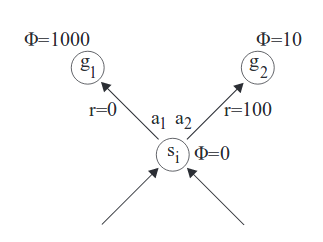
\includegraphics[width=.5\linewidth]{images/reward-shaping-terminal-state}
	\caption{An example that shows why the potential function over terminal state must be 0.}\label{fig:reward-shaping-terminal-state}
\end{figure}

More formally, consider the return of the sequence $\bar{s}$, similarly as Equation \ref{def:expected-discounted-return}:
\begin{equation}\label{def:expected-discounted-return-finite-seq}
\ExpRet(\bar{s}) \defeq \sum_{k=0}^{N-1} \DiscFact^{k}\Reward(s_k, s_{k+1})
\end{equation}

If we apply PBRS, it becomes:
\begin{align}
	\ExpRet_{\Phi}(\bar{s}) &= \sum_{k=0}^{N-1} \DiscFact^{k} (\Reward(s_k, s_{k+1}) + F(s_k, s_{k+1})) \nonumber \\
	&= \sum_{k=0}^{N-1} \DiscFact^{k} (\Reward(s_k, s_{k+1}) + \DiscFact\Phi(s_{k+1}) - \Phi(s_k) ) \nonumber \\
	&= \sum_{k=0}^{N-1} \DiscFact^{k} \Reward(s_k, s_{k+1}) + \sum_{k=1}^{N} \DiscFact^{k}\Phi(s_{k}) - \sum_{k=0}^{N-1} \DiscFact^k\Phi(s_k) \nonumber \\
	&= G(\bar{s}) + \sum_{k=1}^{N-1} \DiscFact^{k}\Phi(s_{k}) + \DiscFact^N\Phi(s_N) - \sum_{k=1}^{N-1} \DiscFact^k\Phi(s_k) - \Phi(s_0) \nonumber \\
	&= G(\bar{s}) + \DiscFact^N\Phi(s_N) - \Phi(s_0) \label{eq:reward-shaping-episodic-terminal-state}
\end{align}
The term $\Phi(s_0)$ cannot alter the policy since does not depend from any action executed; on the other hand, the term $\DiscFact^N\Phi(s_N)$ depends on actions, since the terminal state depends from the previous transitions, hence this term can modify the optimal policy. This happens whenever $\Phi(s_N)\neq 0$, where $s_N$ is any state in which an episode ends, namely goal states, failure states and states where the episode ends due to the time limit exceeded.

A simple solution to this problem is to require that $\Phi(s_N)=0$ whenever the reinforcement learning trajectory is terminated at state $s_N$. Notice that if in other trajectories the same $s_N$ is visited, $\Phi(s_N)$ might be different from 0. The only requirement is that if $s$ is a terminal state, then $\Phi(s) = 0$.

\medskip
\begin{example}\label{exa:reward-shaping-gridworld}
	Recalling Example \ref{exa:gridworld}, we can apply PBRS by defining a potential function that measures how far the agent is from the goal. As heuristic, we can use the \emph{Manhattan distance} between the current position and the goal state. More formally, considering $s_{34}$ the goal state and $s_{ij}$ the current state, we define:
	\[
	\Phi(s) = - [(3 - i) + (4 - j)]
	\]
	It is easy to see that the nearer the agent to the goal state, the higher the potential function evaluated in the state of the agent. For instance, if the current state is $s_{11}$, $\Phi(s_{11}) = - 5$, whereas in $s_{33}$ (which is nearer to the goal), $\Phi(s_{33}) = -1$. 
	With this definition, transition from $s_{11}$ to $s_{12}$ (which makes the agent closer to the goal) evaluates $F(s_{11}, s_{12}) = \Phi(s_{12}) - \Phi(s_{11}) = - 4 - (- 5) = + 1$, whereas for transition $s_{33}\to s_{32}$ (which makes the agent more distant to the goal), $F(s_{33}, s_{32}) = (- 2) - (- 1) = - 1$. 
	
\end{example}

\medskip
In the following sections, we will take into account the topics just described in designing a reward shaping strategy for our setting.

\section{Off-line Reward shaping over $\automaton_\varphi$}\label{sect:off-line-reward-shaping}
In this part we propose an automatic way to apply reward shaping in the setting presented in Section \ref{sect:rl-for-llf-goals}.
Recall that the state space of $\MDPagent^{new}$ is $Q_1\times \dots Q_m \times \States$, where $Q_i$ is the set of states of $\automaton_{\varphi_i}$, the automaton associated to the \LLf formula $\varphi_i$ (see Section \ref{sect:llf2automata}).

The basic intuition about our approach is that \emph{every step toward the satisfaction of a goal formula $\varphi_i$ should be rewarded}, analogously as it is done in reward shaping for classical goals (see Example \ref{exa:reward-shaping-gridworld}). Hence, for a given temporal specification $\varphi_i$ we should assign to every $q\in Q_i$ a potential function that is, to some extent, inversely proportional to the distance from any final state.

Given a (minimal) automaton $\automaton_{\varphi}$ from a \LLf formula $\varphi$ and its associated reward $r$, Algorithm \ref{alg:static-reward-shaping} shows how the potential function is build from $\automaton_{\varphi}$. This operation is made \emph{off-line}, i.e. before the learning process. Then we associate automatically to the states of the \DFA a potential function $\Phi(q)$ whose value decreases proportionally with the minimum distance between the automaton state $q$ and any accepting state. By construction, potential-based reward shaping with this definition of the potential function gives a positive reward when the agent performs an action leading to a $q'$ that is one step closer to an accepting state, and a negative one in the opposite case. Notice that, by construction, $G(\bar{s}) = G_\Phi(\bar{s})$, where $G_\Phi$ is defined in Equation \ref{eq:reward-shaping-episodic-terminal-state}. Indeed, $\DiscFact^N\Phi(s_N) = 0$ because we take into account the issue explained in Section \ref{sect:PBRS-no-gamma}, and $\Phi(s_0) = 0$ by construction of the Algorithm \ref{alg:static-reward-shaping}.

\begin{algorithm}
	\caption{Static Reward Shaping over $\automaton_{\varphi}$}
	\label{alg:static-reward-shaping}
	\begin{algorithmic}[1]
		\State $\mathbf{input}$: (minimal) automaton $\automaton_\varphi$, reward $r$
		\State $\mathbf{output}$: potential function $\Phi: Q\to \Reals$
		
		\State Let $sink$ be the sink state after the completion of $\automaton_{\varphi}$
		\State Let $n_{q_0}$ be minimum number of hops to reach an accepting state from $q_0$ \label{alg-line:q0-distance}
		\For{$q\in Q$}:
			\State Let $n_q$ be minimum number of hops to reach an accepting state from $q$ \label{alg-line:q-distance}
			
			\If{$n_{q_0} \neq 0$} \Comment i.e. if $q_0$ is NOT an accepting state
				\State $\Phi(q) \gets \frac{n_{q_0} - n_q}{n_{q_0}} \cdot r$
			\Else	
				\State $\Phi(q) \gets (n_{q_0} - n_q) \cdot r$
			\EndIf

		\EndFor
		
		\State Let $n_{max}$ the maximum number of hops  to reach an accepting state \label{alg-line:max-distance}
		\State $\Phi(sink) \gets \frac{n_{q_0} - n_{max}}{n_{q_0}} \cdot r \ \mathbf{if}\  n_{q_0}\neq 0 \ \mathbf{else}\  (n_{q_0} - n_{max}) \cdot r$ 
		\State \Return $\Phi$
 	\end{algorithmic}

\end{algorithm}

In the actual implementation of the Algorithm \ref{alg:static-reward-shaping}, $\Phi(q)$ can be computed  by least-fix point over the automaton $\automaton_\varphi$, i.e. starting from the accepting states and then explore the states from the nearest to the farthest ones.

\section{On-The-Fly Reward shaping }
Reward shaping can also be used when the \DFAs of the \LTLf /\LDLf formulas are constructed \emph{on-the-fly} \citep{AAAI1817342} so as to avoid to compute the entire automaton off-line. To do so we can rely on dynamic reward shaping (see Section \ref{sect:DPBRS}).
The idea is to build $\automaton_{\varphi}$ progressively while learning. During the learning process, at every step, the value of the fluents $\ell \in \L$ is observed and the successor state $q'$ of the current state $q$ of the \DFA on-the-fly is computed. 
Then, the transition and the new state just observed are added into the built automaton at time $t$, $\automaton_{\varphi, t}$, yielding $\automaton_{\varphi, t'}$. The potential function $\Phi$ for $\automaton_{\varphi, t'}$ is recomputed for the new version of the automaton. In this case, the shaping function takes the following form: 
\begin{equation}
F(q, t, a, q', t') = \Phi(q', t') - \Phi(q, t)
\end{equation}
i.e. the dynamic reward shaping in Equation \ref{eq:DPBSF} but taking into account the issue presented in Section \ref{sect:PBRS-no-gamma}
where $\Phi(q, t)$ is a variant of the off-line case, but computed on the automaton $\automaton_{\varphi, t}$. In the following we explain how $\Phi$ in the on-the-fly case differs from the one shown in Section \ref{sect:off-line-reward-shaping}.

\subsubsection{Details about $\Phi(q, t)$}
There is an important issue which has not yet been pointed out. In the \emph{off-line} variant described in Section \ref{sect:off-line-reward-shaping}, we apply reward shaping at every transition by knowing the full automaton $\automaton_\varphi$; however, in the \emph{on-the-fly variant}, at the beginning of the learning task we have an "empty" automaton, i.e. only the initial state with no transition from it. 
Let assume that after an action the automaton makes a move from the initial state. How can we assign a positive/negative shaping reward on the transition if we do not know the goodness of the transition?
And if during a simulation we discover an accepting state, there could be a nearer accepting state that has not yet been discovered, but in order to reach it we should first discover other intermediate states. How to allow the agent to discover it while not fixing on the only known accepting states?

It is clear that, the farther the learning task goes, the more accurate will be the shaping rewards, because every observed transition of the automaton during the activity of the agent is stored and eventually the entire automaton will be explored. However, some paths ending in an accepting state are not fully explored, so how to encourage the agent, in our setting, to explore those paths?

In order to determine $\Phi(s, t)$ for a given $A_{\varphi, t}$, we consider the same computations of Algorithm \ref{alg:static-reward-shaping} but \emph{considering the leaves (wrt the initial state) of the automaton as accepting state}. In this way, even if a path does not end in an accepting state, its following is still rewarded. It could be \emph{wrongly rewarded}, since the path might lead to a failure state. However, the dynamic reward shaping theory states that until the potential-based condition is preserved, also the optimal and near-optimal solutions are preserved; moreover, eventually, once the final state of the path is discovered, the reward for that path will assume the right values.

The search for the leaves states is done through Depth-First Search, while the computation is the same of the Algorithm \ref{alg:static-reward-shaping}.

\medskip
It is easy to see that:

\begin{theorem}
	Automata-based reward shaping, both in off-line and on-the-fly variants, preserves optimality and near-optimality of the MDP solutions.
\end{theorem}
\begin{proof} For the off-line case, the shaping-reward function $\Phi$ is, by construction, potential based, hence fulfilling the premises of theorems in \citep{Ng:1999:PIU:645528.657613} and \citep{Grzes:2017:RSE:3091125.3091208}.
	Also for the on-the-fly variant, we observe that our construction is compliant with the requirements defined in \citep{Devlin:2012:DPR:2343576.2343638}.
\end{proof}